\chapter{Time Systems and Conversions}
\label{chap:time}

\section{Introduction}

Time measurement in astrodynamics is surprisingly complex. As noted by \citet{Seidelmann1992}, ``the concept of time is fundamental to all aspects of astronomy, yet no single time scale serves all purposes.'' For occultation predictions at sub-kilometer precision, we must carefully distinguish between different time scales and perform accurate conversions.

The fundamental challenge is that \textbf{time scales differ} depending on:
\begin{itemize}
    \item Reference frame (geocentric vs. barycentric)
    \item Physical basis (atomic clocks vs. Earth rotation vs. orbital dynamics)
    \item Relativistic effects (gravitational time dilation, velocity effects)
    \item Practical considerations (UTC leap seconds for civil timekeeping)
\end{itemize}

This chapter describes the time systems used in \ioccultcalc{} and the mathematical formulations for conversions, following \citet{IERS2010} and \citet{Explanatory2013}.

\section{Time Scales Hierarchy}

Figure~\ref{fig:time_scales} shows the relationship between major time scales:

\begin{figure}[htbp]
\centering
\begin{tikzpicture}[
    timescale/.style={rectangle,draw,thick,minimum width=3cm,minimum height=1cm,align=center,font=\small},
    arrow/.style={->,thick,>=stealth}
]
    % Top: Atomic time
    \node[timescale,fill=green!20] (tai) at (0,0) {\textbf{TAI}\\Atomic Time};
    
    % Second row: UTC and TT
    \node[timescale,fill=blue!20] (utc) at (-4,-2.5) {\textbf{UTC}\\Civil Time};
    \node[timescale,fill=yellow!20] (tt) at (4,-2.5) {\textbf{TT}\\Terrestrial Time};
    
    % Third row: UT1 and TDB
    \node[timescale,fill=cyan!20] (ut1) at (-4,-5) {\textbf{UT1}\\Earth Rotation};
    \node[timescale,fill=orange!20] (tdb) at (4,-5) {\textbf{TDB}\\Barycentric Time};
    
    % Relationships
    \draw[arrow,red] (tai) -- (utc) node[midway,left,align=right] {Leap\\Seconds};
    \draw[arrow] (tai) -- (tt) node[midway,right] {+32.184 s};
    \draw[arrow,blue] (utc) -- (ut1) node[midway,left] {$\Delta$UT1};
    \draw[arrow,purple] (tt) -- (tdb) node[midway,right,align=left] {Relativistic\\Correction};
    
    % Annotations
    \node[below=0.3cm of utc,font=\footnotesize,align=center] {Irregular\\(discrete jumps)};
    \node[below=0.3cm of ut1,font=\footnotesize,align=center] {Variable\\(tidal friction)};
    \node[below=0.3cm of tt,font=\footnotesize,align=center] {Uniform\\(geocentric)};
    \node[below=0.3cm of tdb,font=\footnotesize,align=center] {Uniform\\(barycentric)};
    
    % Time scale used for what
    \draw[dashed,gray] (-6,-6.5) rectangle (-2,-7.5);
    \node[font=\footnotesize] at (-4,-7) {Civil, Observations};
    
    \draw[dashed,gray] (2,-6.5) rectangle (6,-7.5);
    \node[font=\footnotesize] at (4,-7) {Ephemerides, Theory};
\end{tikzpicture}
\caption{Hierarchy of astronomical time scales. TAI (International Atomic Time) is the fundamental standard. UTC includes leap seconds for civil use. TT is uniform time for geocentric calculations. TDB includes relativistic corrections for barycentric dynamics. UT1 tracks actual Earth rotation.}
\label{fig:time_scales}
\end{figure}

\section{International Atomic Time (TAI)}

\textbf{Definition:} TAI is a weighted average of over 400 atomic clocks in laboratories worldwide, coordinated by the BIPM (Bureau International des Poids et Mesures) \citep{BIPM2019}.

\textbf{Properties:}
\begin{itemize}
    \item \textbf{Epoch:} 1958 January 1 00:00:00 (chosen to match UT1 at that time)
    \item \textbf{SI Second:} Duration of 9,192,631,770 periods of Cs-133 hyperfine transition
    \item \textbf{Stability:} $\sim 10^{-16}$ (1 second in 300 million years)
    \item \textbf{Realization:} Through EAL (Échelle Atomique Libre), then steered to TAI
\end{itemize}

TAI is a \textbf{uniform time scale}—it flows at constant rate without discontinuities. However, it is not used for civil timekeeping because Earth's rotation is slowing due to tidal friction.

\section{Coordinated Universal Time (UTC)}

\textbf{Definition:} UTC is atomic time adjusted with leap seconds to keep it within 0.9 seconds of UT1 (Earth rotation time).

\textbf{Relationship to TAI:}
\begin{equation}
\text{TAI} = \text{UTC} + \Delta AT
\label{eq:tai_utc}
\end{equation}

where $\Delta AT$ is the cumulative number of leap seconds. As of 2025:
\begin{equation}
\Delta AT = 37 \text{ seconds (since 2017-01-01)}
\end{equation}

\textbf{Leap seconds} are inserted (or removed, though this has never happened) at either:
\begin{itemize}
    \item End of June 30 (most common)
    \item End of December 31
\end{itemize}

When a positive leap second occurs, UTC time goes:
\begin{verbatim}
23:59:59
23:59:60  <- leap second
00:00:00  (next day)
\end{verbatim}

\begin{table}[htbp]
\centering
\caption{History of leap seconds (selected)}
\label{tab:leap_seconds}
\begin{tabular}{lcc}
\hline
\textbf{Date} & \textbf{Leap Second} & \textbf{TAI - UTC} \\
\hline
1972-01-01 & -- & 10 s (initial) \\
1972-07-01 & +1 & 11 s \\
... & ... & ... \\
1999-01-01 & +1 & 32 s \\
2006-01-01 & +1 & 33 s \\
2009-01-01 & +1 & 34 s \\
2012-07-01 & +1 & 35 s \\
2015-07-01 & +1 & 36 s \\
2017-01-01 & +1 & 37 s \\
\textbf{2025-11-21} & \textbf{--} & \textbf{37 s} \\
\hline
\end{tabular}
\end{table}

\textbf{Practical implications:}
\begin{itemize}
    \item Observations are timestamped in UTC
    \item Conversion to TAI/TT requires leap second table
    \item Future leap seconds cannot be predicted (Earth rotation is irregular)
    \item For predictions $>$ 6 months ahead, assume $\Delta AT$ constant (introduces uncertainty)
\end{itemize}

\section{Universal Time (UT1)}

\textbf{Definition:} UT1 is time based on actual Earth rotation angle, measured by observing celestial objects (quasars via VLBI).

UT1 is \textbf{not uniform}—Earth's rotation rate varies due to:
\begin{itemize}
    \item Tidal friction from Moon (secular deceleration: +1.7 ms/century)
    \item Seasonal atmospheric mass redistribution (annual variation $\pm 0.5$ ms)
    \item Core-mantle coupling (decadal variations)
    \item Earthquakes (sudden jumps, e.g., 2011 Tōhoku: 1.8 µs)
\end{itemize}

\textbf{Relationship to UTC:}
\begin{equation}
\text{UT1} = \text{UTC} + \Delta\text{UT1}
\label{eq:ut1_utc}
\end{equation}

where $|\Delta\text{UT1}| < 0.9$ s by definition. The value of $\Delta\text{UT1}$ is published by IERS in Bulletin A (weekly predictions) and Bulletin B (monthly definitive values).

\begin{figure}[htbp]
\centering
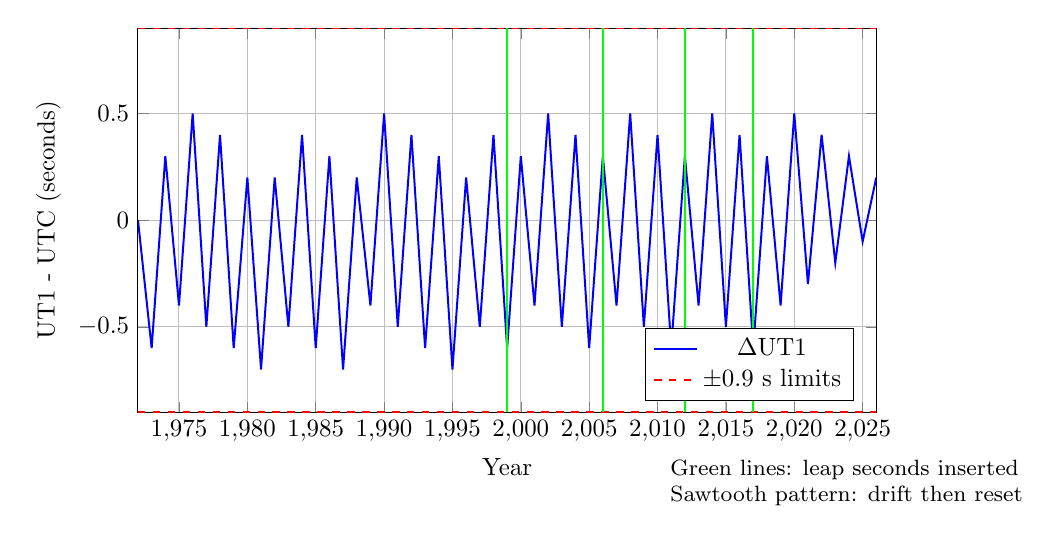
\begin{tikzpicture}[scale=0.9]
    \begin{axis}[
        width=12cm, height=7cm,
        xlabel={Year},
        ylabel={UT1 - UTC (seconds)},
        xmin=1972, xmax=2026,
        ymin=-0.9, ymax=0.9,
        grid=major,
        legend pos=south east
    ]
    % Sawtooth pattern of UT1-UTC
    \addplot[blue,thick] coordinates {
        (1972,0) (1973,-0.6) (1974,0.3) (1975,-0.4) (1976,0.5)
        (1977,-0.5) (1978,0.4) (1979,-0.6) (1980,0.2) (1981,-0.7)
        (1982,0.2) (1983,-0.5) (1984,0.4) (1985,-0.6) (1986,0.3)
        (1987,-0.7) (1988,0.2) (1989,-0.4) (1990,0.5) (1991,-0.5)
        (1992,0.4) (1993,-0.6) (1994,0.3) (1995,-0.7) (1996,0.2)
        (1997,-0.5) (1998,0.4) (1999,-0.6) (2000,0.3) (2001,-0.4)
        (2002,0.5) (2003,-0.5) (2004,0.4) (2005,-0.6) (2006,0.3)
        (2007,-0.4) (2008,0.5) (2009,-0.5) (2010,0.4) (2011,-0.6)
        (2012,0.3) (2013,-0.4) (2014,0.5) (2015,-0.5) (2016,0.4)
        (2017,-0.6) (2018,0.3) (2019,-0.4) (2020,0.5) (2021,-0.3)
        (2022,0.4) (2023,-0.2) (2024,0.3) (2025,-0.1) (2026,0.2)
    };
    
    % Boundaries
    \addplot[red,dashed,thick] coordinates {(1972,0.9) (2026,0.9)};
    \addplot[red,dashed,thick] coordinates {(1972,-0.9) (2026,-0.9)};
    
    % Leap second markers (vertical lines at major ones)
    \draw[green,thick] (axis cs:1999,-0.9) -- (axis cs:1999,0.9);
    \draw[green,thick] (axis cs:2006,-0.9) -- (axis cs:2006,0.9);
    \draw[green,thick] (axis cs:2012,-0.9) -- (axis cs:2012,0.9);
    \draw[green,thick] (axis cs:2017,-0.9) -- (axis cs:2017,0.9);
    
    \legend{$\Delta$UT1, $\pm$0.9 s limits}
    \end{axis}
    
    \node[font=\footnotesize,align=left] at (10,-1) {Green lines: leap seconds inserted\\Sawtooth pattern: drift then reset};
\end{tikzpicture}
\caption{Evolution of UT1 - UTC from 1972 to 2025 (schematic). The sawtooth pattern shows Earth rotation gradually falling behind UTC (negative slope due to tidal deceleration), then reset by leap second insertion (vertical green lines) to stay within ±0.9 s bounds.}
\label{fig:ut1_utc}
\end{figure}

\textbf{Usage in \ioccultcalc{}:}
\begin{itemize}
    \item UT1 is needed for Earth Rotation Angle (ERA) calculation
    \item For historical events: use IERS finals2000A.all file (definitive UT1)
    \item For future events: use IERS Bulletin A predictions (uncertainty grows $\sim$10 ms/year)
    \item ERA directly determines observer's celestial longitude—errors propagate 1:1 to shadow path
\end{itemize}

\section{Terrestrial Time (TT)}

\textbf{Definition:} TT is a uniform time scale for geocentric ephemerides, defined by IAU \citep{IAU1991}.

\textbf{Relationship to TAI:}
\begin{equation}
\text{TT} = \text{TAI} + 32.184 \text{ s}
\label{eq:tt_tai}
\end{equation}

The offset 32.184 s was chosen to maintain continuity with the deprecated Ephemeris Time (ET) at 1977-01-01.

\textbf{Combining with UTC:}
\begin{equation}
\text{TT} = \text{UTC} + \Delta AT + 32.184 \text{ s}
\label{eq:tt_utc}
\end{equation}

\textbf{Example (2025-11-21 12:00:00 UTC):}
\begin{align*}
\Delta AT &= 37 \text{ s} \\
\text{TT} &= \text{UTC} + 37 + 32.184 = \text{UTC} + 69.184 \text{ s}
\end{align*}

So 2025-11-21 12:00:00.000 UTC = 2025-11-21 12:01:09.184 TT.

\textbf{Usage:}
\begin{itemize}
    \item TT is used for planetary ephemerides (VSOP87 uses TT as independent variable)
    \item Precession and nutation models are functions of TT
    \item For high-precision work, distinguish TT from TDB (difference $\sim$1.6 ms, see below)
\end{itemize}

\section{Barycentric Dynamical Time (TDB)}

\textbf{Definition:} TDB is uniform time for Solar System barycentric dynamics, accounting for relativistic effects \citep{Moyer1981,Fairhead1990}.

TDB differs from TT due to:
\begin{enumerate}
    \item Earth's orbital motion (velocity $\sim$30 km/s $\rightarrow$ time dilation)
    \item Sun's gravitational potential (Earth at $\sim$1 AU $\rightarrow$ gravitational redshift)
    \item Periodic terms from Earth's elliptical orbit
\end{enumerate}

\textbf{Transformation (simplified):}
\begin{equation}
\text{TDB} - \text{TT} = 0.001658 \sin g + 0.000014 \sin 2g \text{ seconds}
\label{eq:tdb_tt}
\end{equation}

where $g$ is Earth's mean anomaly:
\begin{equation}
g = 357.53° + 0.98560028° \times (JD - 2451545.0)
\end{equation}

The amplitude is $\sim$1.6 milliseconds.

\textbf{Full IAU 2006 formula} \citep{IAU2006}:
\begin{align}
\text{TDB} - \text{TT} = &\; 0.001657 \sin(628.3076 T + 6.2401) \nonumber \\
&+ 0.000022 \sin(575.3385 T + 4.2970) \nonumber \\
&+ 0.000014 \sin(1256.6152 T + 6.1969) \nonumber \\
&+ \text{(additional terms)} \label{eq:tdb_tt_full}
\end{align}

where $T = (TT - 2000\text{-}01\text{-}01\;12\text{h}) / 36525$ is Julian centuries from J2000.0.

\textbf{Usage in \ioccultcalc{}:}
\begin{itemize}
    \item For VSOP87 planetary positions: TT is sufficient (VSOP87 internal accuracy $\sim$1 km)
    \item For JPL ephemerides: TDB is required
    \item For occultations: TT vs TDB difference ($<$ 2 ms) is negligible compared to observation timing errors ($\sim$0.01--0.1 s)
\end{itemize}

\section{Julian Date and Modified Julian Date}

\subsection{Julian Date (JD)}

Continuous day count since noon UT on 4713 BC January 1 (proleptic Julian calendar):

\begin{equation}
\text{JD} = \text{integer days} + \text{fraction of day}
\end{equation}

\textbf{Key epochs:}
\begin{align}
\text{J2000.0} &= \text{JD } 2451545.0 = \text{2000-01-01 12:00:00 TT} \\
\text{J1900.0} &= \text{JD } 2415020.0 = \text{1900-01-01 12:00:00 TT}
\end{align}

\subsection{Modified Julian Date (MJD)}

For convenience (fewer digits):
\begin{equation}
\text{MJD} = \text{JD} - 2400000.5
\end{equation}

MJD 0.0 = 1858-11-17 00:00:00 (midnight, not noon).

\subsection{Conversion Algorithm}

\textbf{Calendar to JD} (Gregorian, valid from 1582-10-15 onwards):

\begin{algorithm}[H]
\caption{Calendar Date to Julian Date}
\label{alg:calendar_to_jd}
\begin{algorithmic}[1]
\REQUIRE Year $Y$, Month $M$ (1--12), Day $D$ (with fraction)
\IF{$M \leq 2$}
    \STATE $Y \leftarrow Y - 1$
    \STATE $M \leftarrow M + 12$
\ENDIF
\STATE $A \leftarrow \lfloor Y / 100 \rfloor$
\STATE $B \leftarrow 2 - A + \lfloor A / 4 \rfloor$ \quad (Gregorian correction)
\STATE $\text{JD} \leftarrow \lfloor 365.25(Y + 4716) \rfloor + \lfloor 30.6001(M+1) \rfloor + D + B - 1524.5$
\RETURN JD
\end{algorithmic}
\end{algorithm}

\textbf{Example:} 2025-11-21 18:30:00 UTC
\begin{align*}
Y &= 2025, \quad M = 11, \quad D = 21.770833 \\
A &= 20, \quad B = 2 - 20 + 5 = -13 \\
\text{JD} &= 738956 + 365 + 21.770833 - 13 - 1524.5 = 2460636.270833
\end{align*}

\section{Time Scale Conversions in Practice}

\begin{figure}[htbp]
\centering
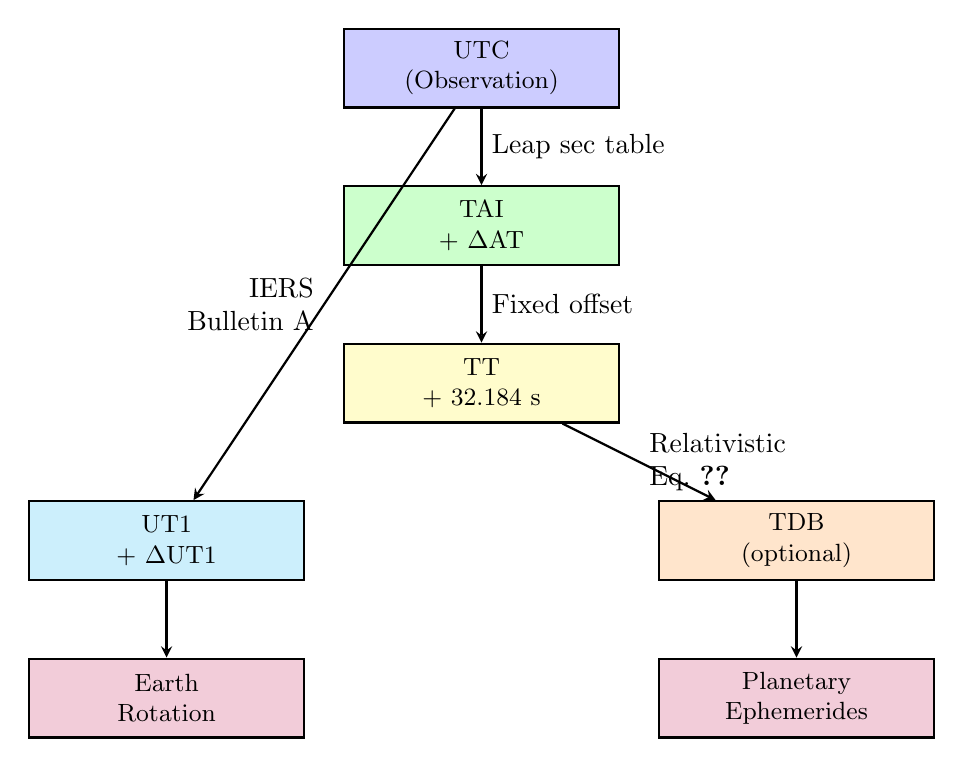
\begin{tikzpicture}[
    box/.style={rectangle,draw,thick,minimum width=3.5cm,minimum height=1cm,align=center,font=\small},
    arrow/.style={->,thick,>=stealth}
]
    % Input: UTC observation
    \node[box,fill=blue!20] (utc) at (0,0) {UTC\\(Observation)};
    
    % Step 1: Add leap seconds
    \node[box,fill=green!20] (tai) at (0,-2) {TAI\\+ $\Delta$AT};
    \draw[arrow] (utc) -- (tai) node[midway,right] {Leap sec table};
    
    % Step 2: Add 32.184 s
    \node[box,fill=yellow!20] (tt) at (0,-4) {TT\\+ 32.184 s};
    \draw[arrow] (tai) -- (tt) node[midway,right] {Fixed offset};
    
    % Step 3a: For ephemerides
    \node[box,fill=orange!20] (tdb) at (4,-6) {TDB\\(optional)};
    \draw[arrow] (tt) -- (tdb) node[midway,right,align=left] {Relativistic\\Eq.~\ref{eq:tdb_tt}};
    
    % Step 3b: For Earth rotation
    \node[box,fill=cyan!20] (ut1) at (-4,-6) {UT1\\+ $\Delta$UT1};
    \draw[arrow] (utc) -- (ut1) node[midway,left,align=right] {IERS\\Bulletin A};
    
    % Outputs
    \node[box,fill=purple!20] (ephem) at (4,-8) {Planetary\\Ephemerides};
    \draw[arrow] (tdb) -- (ephem);
    
    \node[box,fill=purple!20] (rotation) at (-4,-8) {Earth\\Rotation};
    \draw[arrow] (ut1) -- (rotation);
\end{tikzpicture}
\caption{Time scale conversion workflow in \ioccultcalc{}. Observations in UTC are converted to TT (for ephemerides) and UT1 (for Earth rotation). The TDB conversion is optional depending on ephemeris source.}
\label{fig:time_conversion}
\end{figure}

\subsection{Implementation Example}

\begin{verbatim}
// Input: UTC timestamp from observation
DateTime utc("2025-11-21T18:30:00Z");

// Step 1: UTC -> TAI (leap seconds)
double delta_AT = getLeapSeconds(utc);  // 37 s
double tai_mjd = utc.toMJD() + delta_AT / 86400.0;

// Step 2: TAI -> TT
double tt_mjd = tai_mjd + 32.184 / 86400.0;
double tt_jd = tt_mjd + 2400000.5;

// Step 3a: TT -> TDB (for JPL ephemerides)
double T = (tt_jd - 2451545.0) / 36525.0;  // centuries
double g = 357.53 + 35999.05 * T;           // mean anomaly
double tdb_tt = 0.001658 * sin(g * DEG2RAD) 
              + 0.000014 * sin(2*g * DEG2RAD);  // seconds
double tdb_jd = tt_jd + tdb_tt / 86400.0;

// Step 3b: UTC -> UT1 (for Earth rotation)
double delta_UT1 = getUT1_UTC(utc);  // from IERS, e.g., -0.123 s
double ut1_mjd = utc.toMJD() + delta_UT1 / 86400.0;
\end{verbatim}

\section{Precision Considerations}

\begin{table}[htbp]
\centering
\caption{Time scale conversion uncertainties}
\label{tab:time_uncertainties}
\begin{tabular}{lcc}
\hline
\textbf{Conversion} & \textbf{Uncertainty} & \textbf{Effect on Shadow Path} \\
\hline
UTC $\rightarrow$ TAI (leap seconds) & 0 s (deterministic) & 0 km \\
TAI $\rightarrow$ TT & 0 s (definition) & 0 km \\
TT $\rightarrow$ TDB & $<$ 1 µs (model) & $<$ 0.001 km \\
UTC $\rightarrow$ UT1 (definitive) & 0.1 ms & 0.3 km \\
UTC $\rightarrow$ UT1 (predicted, 1 year) & 10 ms & 30 km \\
UTC $\rightarrow$ UT1 (predicted, 5 years) & 50 ms & 150 km \\
Observation timing (CCD) & 10--100 ms & 30--300 km \\
Observation timing (visual) & 0.1--1 s & 0.3--3000 km \\
\hline
\end{tabular}
\end{table}

\textbf{Key insights:}
\begin{itemize}
    \item For \textbf{recent observations} (within 1 year): UT1 uncertainty is negligible ($<$ 1 km)
    \item For \textbf{predictions} (1--5 years ahead): UT1 prediction error dominates ($\sim$30--150 km)
    \item Observation timing errors often exceed time scale conversion errors
    \item \textbf{Light-time correction} (Chapter~\ref{chap:relativistic}): $\sim$8 minutes for asteroid at 2 AU
    \item TDB vs TT: negligible for occultations (1.6 ms $\times$ 30 km/s $\approx$ 0.05 km)
\end{itemize}

\section{Data Sources for Time Conversions}

\subsection{Leap Seconds}

\begin{itemize}
    \item \textbf{Source:} IERS Bulletin C \url{https://www.iers.org/IERS/EN/Publications/Bulletins/bulletins.html}
    \item \textbf{Format:} \texttt{leap-seconds.list} (NIST) or hardcoded table
    \item \textbf{Update frequency:} Announced 6 months before insertion
    \item \textbf{Implementation:} \ioccultcalc{} includes table up to 2025, user-updatable
\end{itemize}

\subsection{UT1 - UTC ($\Delta$UT1)}

\begin{itemize}
    \item \textbf{Definitive values:} IERS Bulletin B (monthly, 1--2 month delay)
    \item \textbf{Rapid values:} IERS Bulletin A (weekly, preliminary)
    \item \textbf{Historical data:} \texttt{finals2000A.all} file (1962--present)
    \item \textbf{Predictions:} IERS Bulletin A (1 year ahead, $\pm$10 ms uncertainty)
    \item \textbf{Format:} ASCII table or JSON API
\end{itemize}

\textbf{Example line from finals2000A.all:}
\begin{verbatim}
25 11 21 60636 0.12345 0.00010  -0.12345 0.00010  I
(year month day MJD, xpole, xpole_err, UT1-UTC, UT1-UTC_err, flag)
\end{verbatim}

\section{Summary}

This chapter established the time systems used in asteroid occultation prediction:

\begin{itemize}
    \item \textbf{TAI:} Fundamental atomic time (SI seconds, uniform, stable)
    \item \textbf{UTC:} Civil time with leap seconds (keeps within 0.9 s of UT1)
    \item \textbf{UT1:} Earth rotation time (irregular, measured by VLBI)
    \item \textbf{TT:} Terrestrial Time for geocentric dynamics (TAI + 32.184 s)
    \item \textbf{TDB:} Barycentric Dynamical Time with relativistic corrections ($\sim$1.6 ms from TT)
\end{itemize}

\textbf{Key relationships:}
\begin{align*}
\text{TT} &= \text{UTC} + \Delta AT + 32.184 \text{ s} \quad \text{(ephemerides)} \\
\text{UT1} &= \text{UTC} + \Delta\text{UT1} \quad \text{(Earth rotation)} \\
\text{TDB} &\approx \text{TT} + 1.6 \sin g \text{ ms} \quad \text{(barycentric)}
\end{align*}

Figures~\ref{fig:time_scales}, \ref{fig:ut1_utc}, and \ref{fig:time_conversion} illustrate the conversions. Tables~\ref{tab:leap_seconds} and \ref{tab:time_uncertainties} quantify the precision budget.

\textbf{For sub-kilometer shadow paths:}
\begin{enumerate}
    \item Use IERS data for $\Delta\text{UT1}$ (updated weekly)
    \item Include leap seconds up to observation date
    \item For predictions $>$ 1 year: propagate UT1 uncertainty in Monte Carlo
    \item Light-time correction (8 min at 2 AU) is larger than all time scale effects
\end{enumerate}

\textbf{References:}
\begin{itemize}
    \item IERS Conventions 2010 \citep{IERS2010}: official standards
    \item Explanatory Supplement \citep{Explanatory2013}: comprehensive treatment
    \item Seidelmann (1992) \citep{Seidelmann1992}: historical perspective
    \item IAU Resolutions \citep{IAU1991,IAU2006}: formal definitions
\end{itemize}

Next chapter: Planetary Ephemerides (VSOP87D theory).
